%!TEX root = ../template.tex
%%%%%%%%%%%%%%%%%%%%%%%%%%%%%%%%%%%%%%%%%%%%%%%%%%%%%%%%%%%%%%%%%%%%
%% chapter6_ConclusionsFuture.tex
%% NOVA thesis document file
%%
%% Chapter with the Conclusions and Future Work part
%%%%%%%%%%%%%%%%%%%%%%%%%%%%%%%%%%%%%%%%%%%%%%%%%%%%%%%%%%%%%%%%%%%%

\typeout{NT FILE chapter6_ConclusionsFuture.tex}

\chapter{Conclusions and Future Work}\label{cha:chapter6_ConclusionsFuture}

Considering the impact of robotic devices in the most diverse types of fields (whether scientific or not), their precise development is of great importance, so the definition and implementation of a project in an orderly and careful way is quite valuable.

Agricultural work, surveillance, mapping, etc. performed using robotic devices always brings many advantages, taking into account that the yield obtained turns out to be equal or (often) superior to that of a human being.
Thus, in order to develop a device capable of doing so, the first priority will be the study of all the relevant information available, as well as all the technology known on the subject -- the study of the most relevant GNSS positioning technologies covered in Chapter~\ref{cha:chapter2_SotA} covers this aspect, corresponding to the state of the art.
Having done this, the next step is related to the establishment of requirements to be fulfilled for the system to be developed, so that the solution obtained fulfills all the purposes initially intended -- Section~\ref{sec:III_requirements}. To this end, assimilating a chronological order made up of phases allows an estimate of the interdependencies of each one of them, as well as defining expected deadlines (Tables~\ref{tab:workflow} and~\ref{tab:gantt}).\\

\par Successfully accomplishing complicated, hard, and time-consuming tasks is, without a doubt, something that anyone can be proud of. Nonetheless, envisioning and developing a solution capable of performing them as efficiently as possible is undoubtedly the approach that characterizes an engineer. In addition to providing valuable insights into the known literature on navigation through GNSS services -- most emphatically precise positioning --, this document also presents an estimate of the approach to be taken for the development of the project, as well as the chronological order that is considered the wisest for such.

%           PODE SER USADO NA CONCLUSAO: about RTK
% "Real Time Kinematic technique requires 2 receivers. One of them is stationary and is called "base station", the other one is "rover". The base station measures errors, and knowing that it is stationary transmits corrections to the rover (refer to How RTK works for more information about RTK). Sometimes CORS and NTRIP networks take the place of traditional base stations. They provide accurate absolute position and send corrections over the Internet. Typically the distance between the reference station and local rover shouldn't exceed 10-15 km due to the ionospheric effect. So if the reference station is located too far or simply is absent in the area you will need a local base station. Other advantages of your own base are independence from the Internet connection and lack of NTRIP subscription fees."
% - If the accurate absolute position of the base has been determined only after the job has been done, the offset of the map can be determined and corrected.

1. Calcular para uma charge current de 1020mA e nao de 4000mA -- fazer as contas no excel.
1.1 Initially the expected type of Li-ion cell to work with would be capable of being charged with a charging current of $4,000$mA, however, since the circuit ultimately did not end up with a power consumption greater than 250mA and was never powered by the backup pack for a long time, the cells never needed the full programmed bulk charge current (concept explained further ahead in this section). Therefore, due to practicality concerns,

2. para ter 2-level charging: instalar comparador LM311 e seguir o que diz aqui: https://www.electro-tech-online.com/threads/simple-circuit-to-invert-dc-from-positive-to-negative.141411/

2. This results in a value of R15 of approximately 5.36k$\Omega$, however, at the time of soldering, the closest standard resistor value available was 6.2k$\Omega$, which, when applying the same previous law to a variation of the equivalent circuit of
% Figure~\ref{fig:voltage_divider_1}
results in a voltage between R10 and R15 of approximately 1.15V -- sufficient to drive Q3.

3. Meter condensadores de desacoplamento --> como o modulo 3.3V funciona por pulsos (btw tudo no esquematico é digital), vai existir ruido consideravel quando a tensao for puxada/convertida --> os condensadores de desacoplamento servem para atenuar esse ruido.

4. meter o consumo teorico de todos os componentes -- deu me 1.650 mA??? (é suposto dar 400mA @ 5V como diz em \textbf{RTKBS.MAIN.PWS.040})

5. embora tenha a corrente IRMS (\ref{eq:i_rms}) do condensador C8 da battery, nao usei um condensador eletrolitico de aluminio, mas sim um de ceramica de 20uF



%aquele circuito novo do bq29209:---------------------------------
%bq29209:
\subsection{Battery Balancer}\label{sec:6_BQ29209}
As mentioned in Section~\ref{sec:3212_BQ29209},~\cite{bq29209} provides a typical application circuit for the BQ29209 together with a few application notes. However, that typical application circuit should not be implemented for the new beRTK\textsuperscript{\textregistered}, since the internal system of the BQ29209 can only support cell balancing currents of up to 15mA, which would not cause any kind of reaction within the cells used (INR18650-35E), since their minimum charge current is 68mA. Therefore,~\cite{bq29209} provides another application circuit capable of supporting a cell balancing current higher than 15mA. This implementation is presented in Figure~\ref{fig:BQ29209_circuit_NEW}.
% meter aqui circuito do BQ29209 - NEW:
\begin{figure}[h]
    \centering
    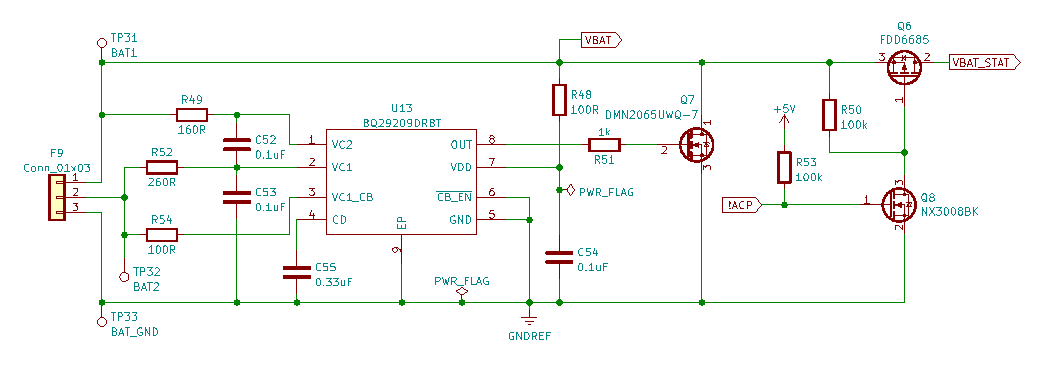
\includegraphics[width=0.3\textwidth]{Chapters/Figures/chapter3/Battery_Balancer.pdf}
    \caption{beRTK\textsuperscript{\textregistered} Base Station's Battery Balancer schematic diagram.}
    \label{fig:BQ29209_circuit_NEW}
\end{figure}

The circuit of Figure~\ref{fig:BQ29209_circuit_NEW} is also valid for a $V_{DD}$ supply voltage ranging from 4V to 10V. This new circuit also ensures that, due to FETs Q3 (NMOS, 2N7002 model) and Q10 (PMOS, FDD6685 model), a higher cell balancing current can safely be established, being it defined by either cell's voltage, along with resistor R4:

\begin{equation}\label{eq:IBAL}
	I_{BAL}=\frac{V_{Cell}}{R4}\,\medskip
\end{equation}

\noindent It should be noted that resistor R54's purpose lies on ensuring that both ``balancing'' FETs will remain off, while cell balancing is not taking place and should be selected with a value above 2k$\Omega$.

\cite{bq29209} clarifies that the BQ29209 ensures cell balancing on the cell that presents the higher voltage of the pack.
Taking into account that recommended cell arrangement sequence (from the bottom of the stack) of GND--Cell1--Cell2 (i.e. from pin 3 to pin 1 of connector F9 -- Figure~\ref{fig:BQ29209_circuit}) was followed, the balancing of Cell1 would start by pulling pin VC1\_CB of BQ29209 to GND, therefore setting PMOS Q10's gate-source voltage at around $-V_{Cell1}$. This would cause a balancing current of $I_{BAL1}=\frac{V_{Cell1}}{R4}$. Conversely, if Cell2 were in need of balancing, VC1\_CB would instead be pulled to $V_{DD}$, thus setting Q3's gate voltage at around $V_{Cell1}+V_{Cell2}$, which translates into a gate-source voltage of approximately $V_{Cell2}$, having the source voltage being set at around $V_{Cell1}$. With this, resorting again to equation (\ref{eq:IBAL}), a cell balancing current of $I_{BAL2}=\frac{V_{Cell2}}{R4}$ results. In order to set a balancing current for each cell that would always surpass the minimum charge current of 68mA, a value of 20$\Omega$ was sized for R4. 

The remaining components' values were selected as to comply with the BQ29209 recommended operating conditions.
%------- fim do new circuit do BQ29209 ----------------------





6. The port is capable of being used as a true USB On-The-Go (OTG) port. While there is no official documentation, some users have had success making this work. The USB\_OTG\_ID pin is used to select between USB host and device that is typically wired to the ID pin of a Micro USB connector. To use this functionality it must be enabled in the OS. If using either as a fixed slave or fixed master, please tie the USB\_OTG\_ID pin to ground. tentei isto e nao deu

7. As mentioned in Section~\ref{sec:3221_CM4_GPIO}, to select one of the alternative functions of a GPIO pin, the GPFSEL0 resgister's address would have to be... -->
    for FSEL9: 011
    for FSEL8: 011
    for FSEL4: 011
why? Because the ZED-F9P pins connected to the CM4's GPIO pins are part of a UART peripheral set on the ZED-F9P module, as it is possible to observe in the circuit of Figure~\ref{fig:ZED-F9P_carrier_board}, along with Section 3.1 of~\cite{ZED_F9P}.

8. % LAN9514:
However, USB has the advantage of allowing hot-swapping, making it useful for mobile peripherals, including drives of various kinds. -- mesmo que digam isto ja é possivel por natureza do USB, eu ainda tentei fazer o que dizia no datahseet do LAN9514 para dar enable ao hot-swapping, mas continuou sem funcionar;
8.1: Meter FIGURE 2-3 do datasheet do LAN9514 e falar do PRTCTL
8.2: falta VDD18USBPLL com capacitor, e com ferrite para VDD18ETHPLL
8.3: o MIC2026A -- power seitching downstream -- serve para garantir que se tem uma limitação de corrente em cada uma das portas; para garantir que não se tem mais que 500 mA em cada porta usb, para não rebentar com os controladores.

9. %cm4:
In Section~\ref{sec:3234_LAN9514}, the lack of implementation of the upstream USB PHY block was addressed. It must be noted that this such block should be implemented in the beRTK\textsuperscript{\textregistered}'s system, since it not only facilitates the OS loading into the CM4, but can also be used to transfer data if needed.

10.
Poder-se-ao colocar mounting holes na main board tambem, de forma a fixa-la na sua casing.

% Dizer isto no final:
no Final de tudo estar bem feito, teria de se demonstrar aquela compliance matrix que apresenta a conclusao de todos os requirements apresentados na Section~\ref{sec:II_Specs}.
